% Star schema figure. Build: xelatex star_schema.tex  ->  star_schema.pdf
\documentclass[border=4pt]{standalone}
\usepackage{fontspec}
\setmainfont{Latin Modern Roman}
\setmonofont{DejaVu Sans Mono}[Scale=0.78]
\usepackage{xcolor}
\usepackage{tikz}
\usetikzlibrary{shapes.multipart,positioning,calc}

\definecolor{factc}{RGB}{214,96,40}
\definecolor{dimc}{RGB}{52,101,164}
\definecolor{bodyc}{RGB}{250,250,250}

\tikzset{
  tbl/.style={rectangle split, rectangle split parts=2, draw=black!60, thick,
    rectangle split part fill={#1, bodyc}, inner xsep=4pt, inner ysep=3pt,
    text width=3.55cm, align=left, font=\ttfamily\scriptsize},
  link/.style={thick, black!55},
  card/.style={font=\bfseries\scriptsize, fill=white, inner sep=1pt}
}
\newcommand{\hd}[1]{\textcolor{white}{\textbf{#1}}}
\newcommand{\pk}{\textcolor{orange!80!black}{\textbf{PK}}}
\newcommand{\fk}{\textcolor{blue!60!black}{\textbf{FK}}}

\begin{document}
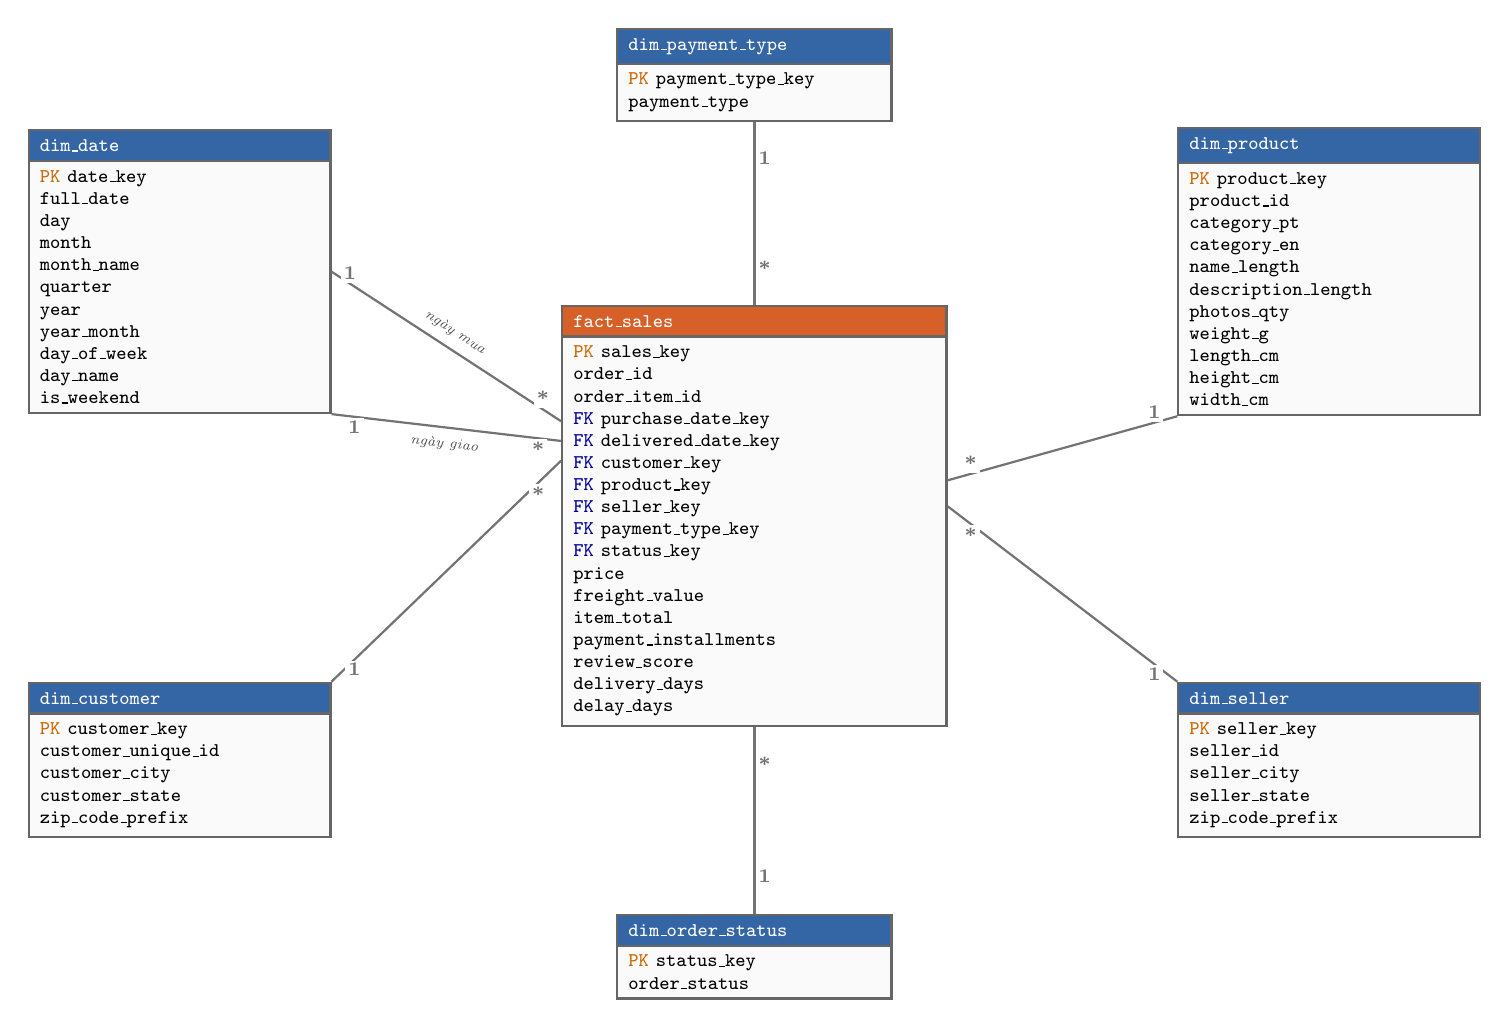
\begin{tikzpicture}

% ---------- FACT (center) ----------
\node[tbl=factc, text width=4.6cm] (fact) at (0,0) {
  \hd{fact\_sales}
  \nodepart{second}
  \pk\ sales\_key\\
  order\_id\\
  order\_item\_id\\
  \fk\ purchase\_date\_key\\
  \fk\ delivered\_date\_key\\
  \fk\ customer\_key\\
  \fk\ product\_key\\
  \fk\ seller\_key\\
  \fk\ payment\_type\_key\\
  \fk\ status\_key\\
  price\\
  freight\_value\\
  item\_total\\
  payment\_installments\\
  review\_score\\
  delivery\_days\\
  delay\_days
};

% ---------- DIMENSIONS ----------
\node[tbl=dimc] (date) at (-7.3,3.1) {
  \hd{dim\_date}
  \nodepart{second}
  \pk\ date\_key\\
  full\_date\\
  day\\
  month\\
  month\_name\\
  quarter\\
  year\\
  year\_month\\
  day\_of\_week\\
  day\_name\\
  is\_weekend
};

\node[tbl=dimc] (cust) at (-7.3,-3.1) {
  \hd{dim\_customer}
  \nodepart{second}
  \pk\ customer\_key\\
  customer\_unique\_id\\
  customer\_city\\
  customer\_state\\
  zip\_code\_prefix
};

\node[tbl=dimc] (prod) at (7.3,3.1) {
  \hd{dim\_product}
  \nodepart{second}
  \pk\ product\_key\\
  product\_id\\
  category\_pt\\
  category\_en\\
  name\_length\\
  description\_length\\
  photos\_qty\\
  weight\_g\\
  length\_cm\\
  height\_cm\\
  width\_cm
};

\node[tbl=dimc] (sell) at (7.3,-3.1) {
  \hd{dim\_seller}
  \nodepart{second}
  \pk\ seller\_key\\
  seller\_id\\
  seller\_city\\
  seller\_state\\
  zip\_code\_prefix
};

\node[tbl=dimc, text width=3.2cm] (pay) at (0,5.6) {
  \hd{dim\_payment\_type}
  \nodepart{second}
  \pk\ payment\_type\_key\\
  payment\_type
};

\node[tbl=dimc, text width=3.2cm] (stat) at (0,-5.6) {
  \hd{dim\_order\_status}
  \nodepart{second}
  \pk\ status\_key\\
  order\_status
};

% ---------- RELATIONSHIPS (1 : *) ----------
% anchor points on the fact border, aligned with the FK rows
\coordinate (fw1) at ($(fact.west)+(0,1.2)$);   % purchase_date_key
\coordinate (fw2) at ($(fact.west)+(0,0.95)$);  % delivered_date_key
\coordinate (fw3) at ($(fact.west)+(0,0.7)$);   % customer_key
\coordinate (fe1) at ($(fact.east)+(0,0.45)$);  % product_key
\coordinate (fe2) at ($(fact.east)+(0,0.12)$);  % seller_key

\draw[link] (date.east) -- node[card,pos=0.08,above]{1} node[card,pos=0.92,above]{*}
  node[midway,above,sloped,font=\itshape\tiny,black!70]{ngày mua} (fw1);
\draw[link] (date.south east) -- node[card,pos=0.1,below]{1} node[card,pos=0.9,below]{*}
  node[midway,below,sloped,font=\itshape\tiny,black!70]{ngày giao} (fw2);
\draw[link] (cust.north east) -- node[card,pos=0.1,below]{1} node[card,pos=0.9,below]{*} (fw3);
\draw[link] (prod.south west) -- node[card,pos=0.1,above]{1} node[card,pos=0.9,above]{*} (fe1);
\draw[link] (sell.north west) -- node[card,pos=0.1,below]{1} node[card,pos=0.9,below]{*} (fe2);
\draw[link] (pay) -- node[card,pos=0.2,right]{1} node[card,pos=0.8,right]{*} (fact.north);
\draw[link] (stat) -- node[card,pos=0.2,right]{1} node[card,pos=0.8,right]{*} (fact.south);

\end{tikzpicture}
\end{document}
